\begin{figure}
	\begin{flushleft}
		\textbf{Users Login Page}:\\
		Since logging into SafeStreets is mandatory, this is the first page that the user will face when the app does not recognizes him. Of course, cookies or sessions could avoid to force the user to login every time.
	\end{flushleft}
	\centering
	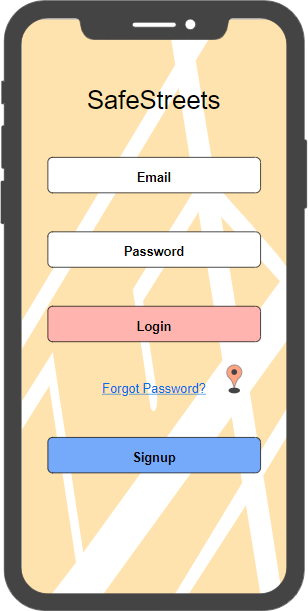
\includegraphics[width=0.6\linewidth]{../RASD/images/mockups/login}
	\caption{SafeStreets Login page.}
\label{fig:login}
\end{figure}
\clearpage
\begin{figure}
	\begin{flushleft}
		\textbf{Officers Login Page}:\\
		Since logging into SafeStreets is mandatory, this is the first page that the officer will face when the portal does not recognizes him. Of course, cookies or sessions could avoid to force the officer to login every time. A Sign-up page is not expected since an officer charged with SafeStreets jobs should also receive an account.
	\end{flushleft}
	\centering
	\makebox[\textwidth][c]{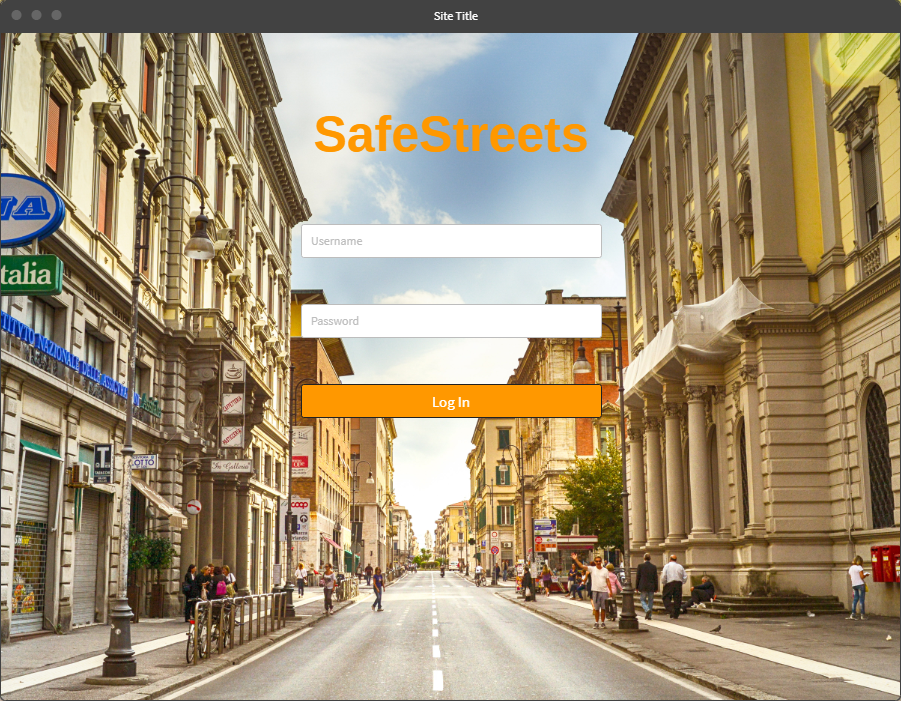
\includegraphics[width=1.4\textwidth]{images/desktopMockups/login}}
	\caption{SafeStreets Login page.}
	\label{fig:login2}
\end{figure}
\clearpage
\begin{figure}
	\begin{flushleft}
		\textbf{Users SignUp Page}:\\
		Since logging into SafeStreets is mandatory, if the user does not have an account he needs to make one. Every field except the photo should be mandatory.
	\end{flushleft}
	\centering
	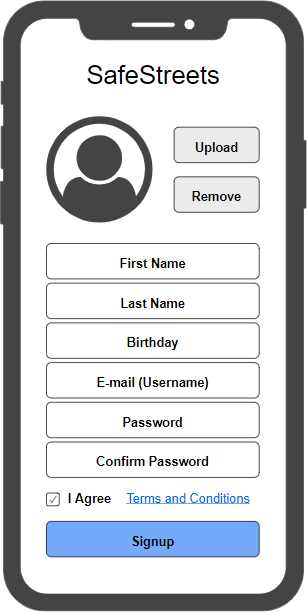
\includegraphics[width=0.6\linewidth]{../RASD/images/mockups/signup}
	\caption{SafeStreets SignUp page.}
	\label{fig:signup}
\end{figure}
\clearpage
\begin{figure}
	\begin{flushleft}
		\textbf{Users Home Page}:\\
		When the user logs into SafeStreets successfully, an home page should be provided with the options for the user to use every functionality of the application.
	\end{flushleft}
	\centering
	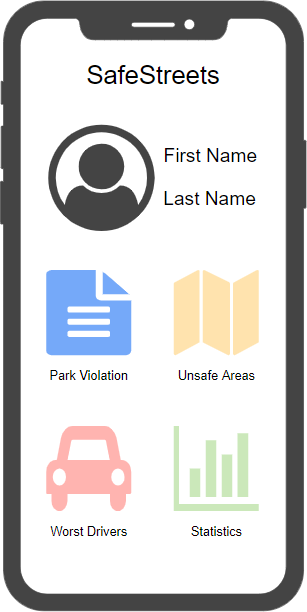
\includegraphics[width=0.6\linewidth]{../RASD/images/mockups/homePage}
	\caption{SafeStreets Home page.}
	\label{fig:home}
\end{figure}
\clearpage
\begin{figure}
	\begin{flushleft}
		\textbf{Officers Home Page}:\\
		When the officer logs into SafeStreets successfully, an home page should be provided with the options for the officer to use every functionality of the application.
	\end{flushleft}
	\centering
	\makebox[\textwidth][c]{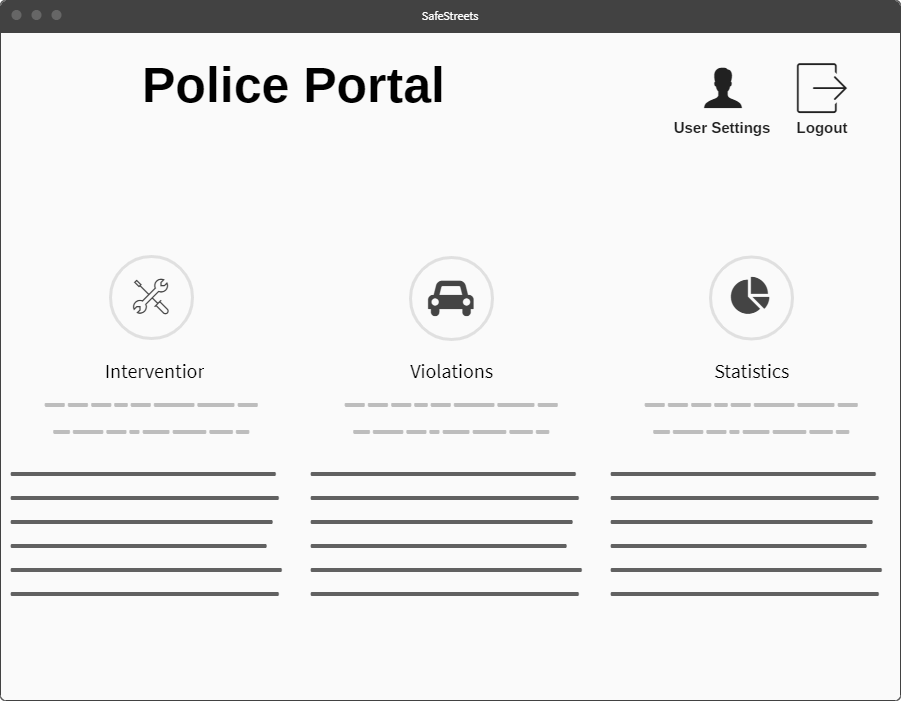
\includegraphics[width=1.4\textwidth]{images/desktopMockups/homePage}}
	\caption{SafeStreets Home page.}
	\label{fig:home2}
\end{figure}
\clearpage
\begin{figure}
	\begin{flushleft}
		\textbf{Users Violation Page}:\\
		If the user wants to send to the officers a parking violation of some sorts a form to be filled is provided. The user can either send a report that will generate an automatic ticket or that will need to be checked by the officers.
	\end{flushleft}
	\centering
	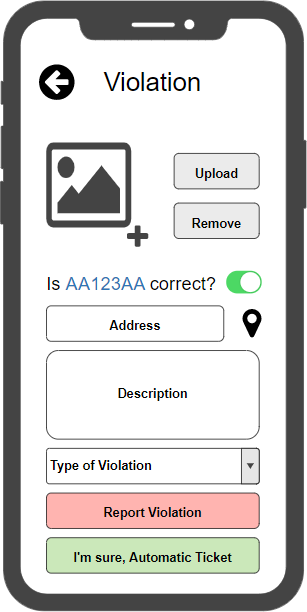
\includegraphics[width=0.6\linewidth]{../RASD/images/mockups/violation}
	\caption{SafeStreets Violation page.}
	\label{fig:violation}
\end{figure}
\clearpage
\begin{figure}
	\begin{flushleft}
		\textbf{Officers Violation Page}:\\
		If the officer needs to check the tickets that the users sent to the portal an interface to handle them is provided. The officer can either abort the violation if it is not considered valid, or file the ticket if the ticket is enough for a fine.
	\end{flushleft}
	\centering
	\makebox[\textwidth][c]{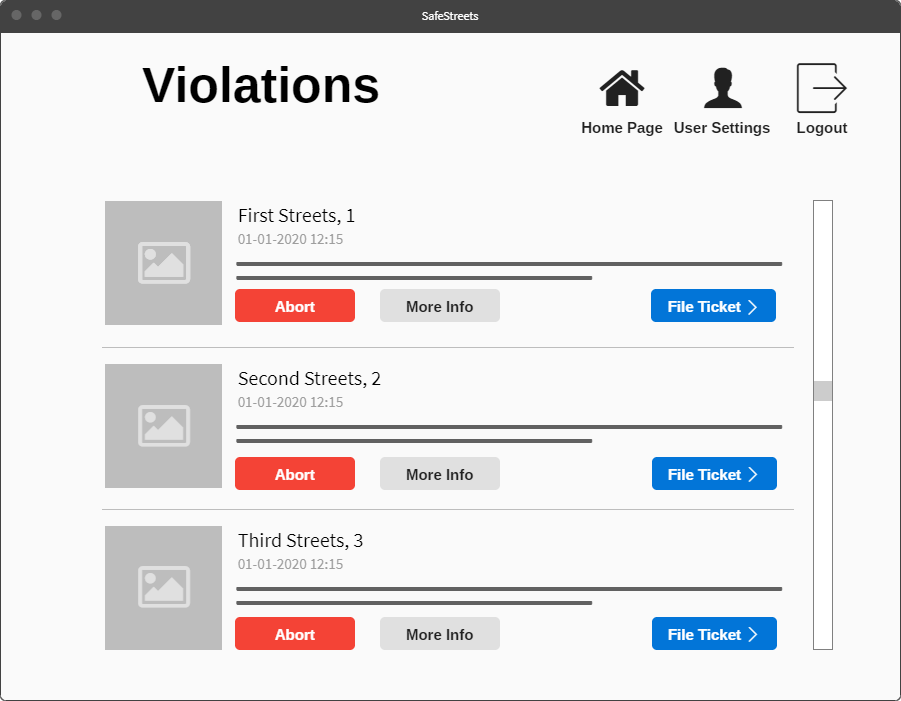
\includegraphics[width=1.4\textwidth]{images/desktopMockups/violation}}
	\caption{SafeStreets Violation page.}
	\label{fig:violation2}
\end{figure}
\clearpage
\begin{figure}
	\begin{flushleft}
		\textbf{Users Unsafe Areas Page}:\\
		If the user wants to see which areas are the most subject to violations, an interface to search among all areas should be implemented.
	\end{flushleft}
	\centering
	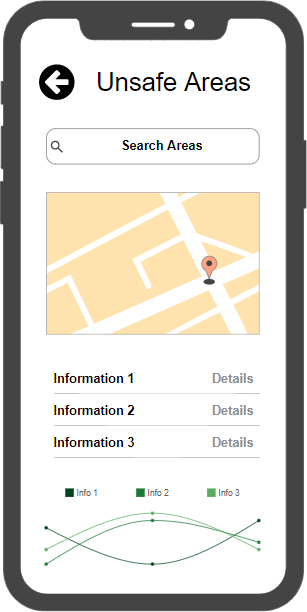
\includegraphics[width=0.6\linewidth]{../RASD/images/mockups/areas}
	\caption{SafeStreets Unsafe Areas page.}
	\label{fig:areas}
\end{figure}
\clearpage
\begin{figure}
	\begin{flushleft}
		\textbf{Users Worst Drivers Page}:\\
		If the user wants to see which vehicles tends to not follow the city rules, an interface that shows this needs to be present in the application.
	\end{flushleft}
	\centering
	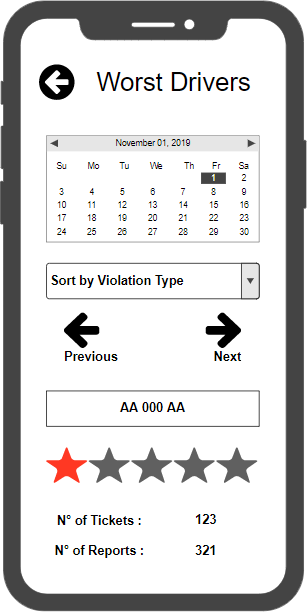
\includegraphics[width=0.6\linewidth]{../RASD/images/mockups/vehicles}
	\caption{SafeStreets Worst Drivers page.}
	\label{fig:vehicles}
\end{figure}
\clearpage
\begin{figure}
	\begin{flushleft}
		\textbf{Officers Suggestions Page}:\\
		If the officer needs to check possible suggestions and interventions for a specific area that the data mining procedures have enlighten, a page that enable this is provided. The officer can given a map select the spots that have a possible intervention to apply and decide if it is a valid or not suggestion.
	\end{flushleft}
	\centering
	\makebox[\textwidth][c]{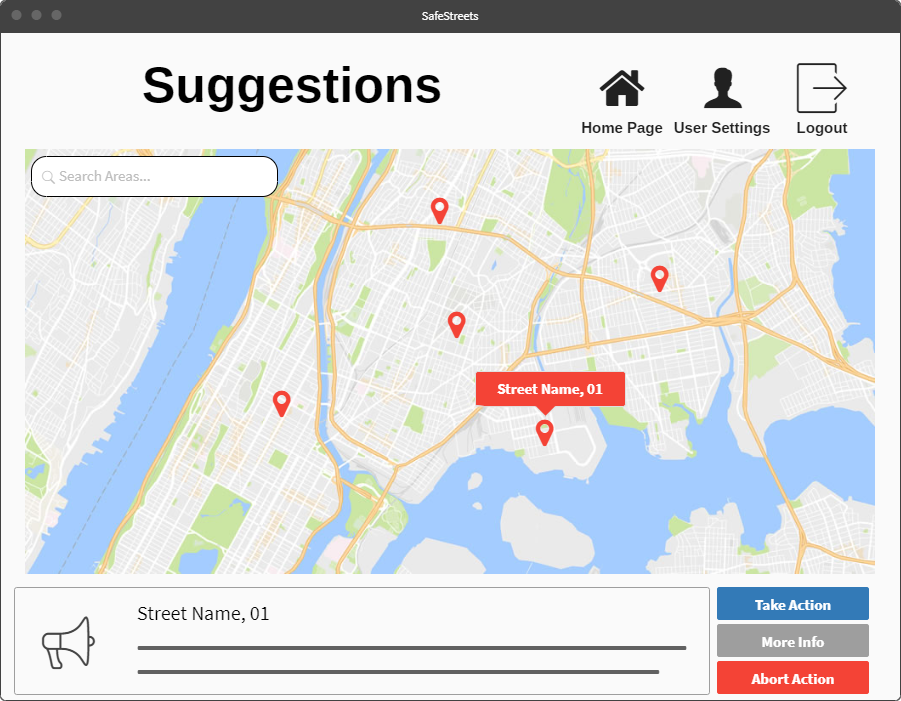
\includegraphics[width=1.4\textwidth]{images/desktopMockups/suggestions}}
	\caption{SafeStreets Statistics page.}
	\label{fig:suggestions}
\end{figure}
\clearpage
\begin{figure}
	\begin{flushleft}
		\textbf{Users Statistics Page}:\\
		A complete page that exhibits all of SafeStreets data in a complete and detailed manner, that also enlightens SafeStreets effectiveness. 
	\end{flushleft}
	\centering
	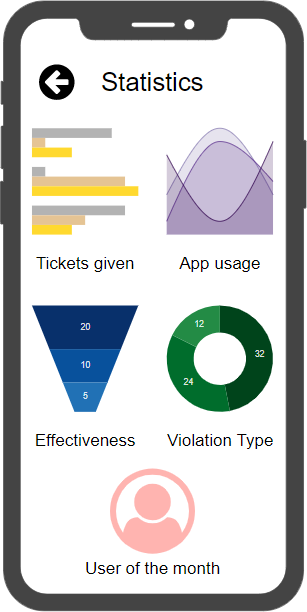
\includegraphics[width=0.6\linewidth]{../RASD/images/mockups/statistics}
	\caption{SafeStreets Statistics page.}
	\label{fig:statistics}
\end{figure}
\clearpage
\begin{figure}
	\begin{flushleft}
		\textbf{Officers Statistics Page}:\\
		A complete page that exhibits all of SafeStreets data in a complete and detailed manner, that also enlightens SafeStreets effectiveness. Within this page the officers have access to the unsafe areas and worst drivers information, as long as more sensitive data such as the detailed information of the owners of the worst car users.
	\end{flushleft}
	\centering
	\makebox[\textwidth][c]{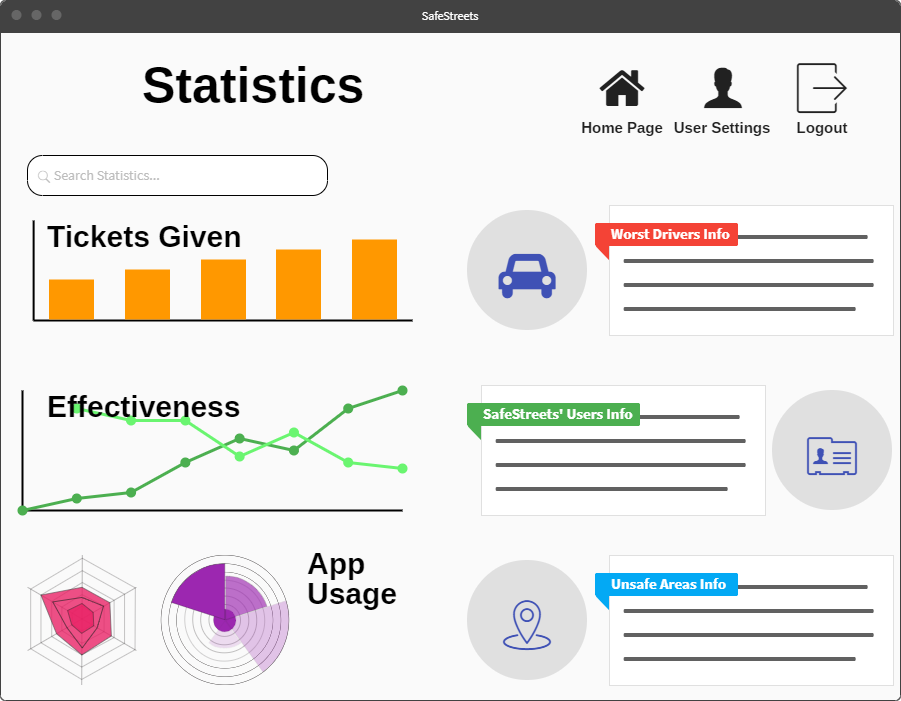
\includegraphics[width=1.4\textwidth]{images/desktopMockups/statistics}}
	\caption{SafeStreets Statistics page.}
	\label{fig:statistics2}
\end{figure}
\clearpage
\begin{figure}
	\begin{flushleft}
		\textbf{User Profile Page}:\\
		If the user wants to change its profile picture or his password, if he wants to check his reports or to logout, he should be able to do all these things. 
	\end{flushleft}
	\centering
	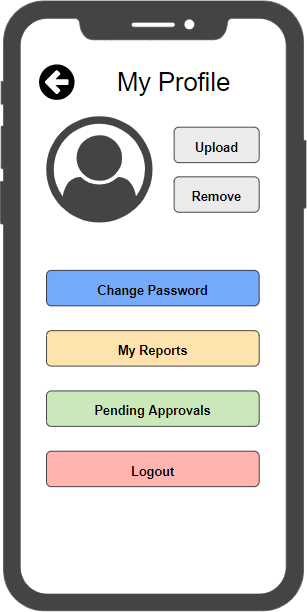
\includegraphics[width=0.6\linewidth]{../RASD/images/mockups/profile}
	\caption{SafeStreets User Profile page.}
	\label{fig:profile}
\end{figure}
\clearpage